\setcounter{section}{3}
\section{\texorpdfstring{$L^p$}{Lp} Spaces}

\begin{note}{Thm 4.5}
    See the proof that $l^p$ is a Banach space \href{https://tech.dafuzhu.com/courses/mit18102/a1/#problem-2}{here}. 
    \[
    l^p: \|x\|_p=\left(
    \sum_{i=1}^n |x_i|^p
    \right)^{1/p},\quad L^p:\|f\|_p=\left(
    \int |f|^p \dif \mu
    \right)^{1/p}
    \]
    In \( \ell^{p} \), the input is a sequence (or vector) \( x=\{x_{i}\}_{i \geq 1} \). In \( L^{p} \), the input is an equivalence class of measurable functions \( [f] \).
\end{note}

\begin{note}{Def 4.10}
    Absolute continuity $v\ll \mu$ is an analogy from real analysis. $\Delta x\to 0\implies \Delta f\to 0$; $\mu(A)=0\implies v(A)=0$. $f$ is controlled by $x$ and $v$ is controlled by $\mu$. See Fig \ref{fig:def4.10}.
    \begin{figure}[htbp]
        \centering
        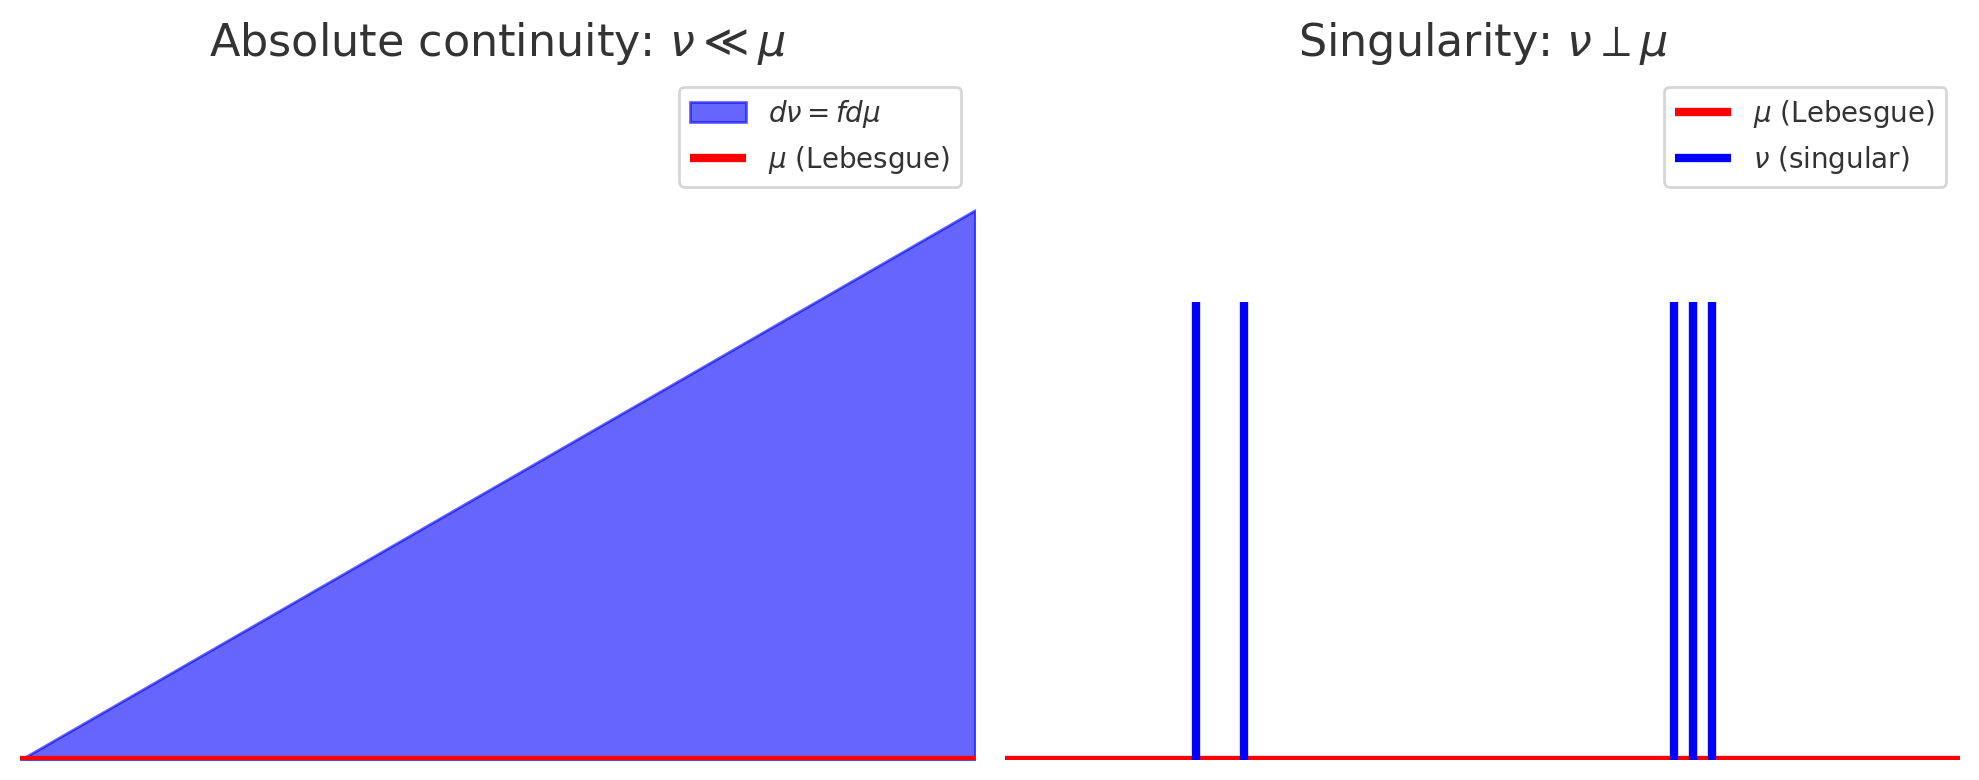
\includegraphics[width=0.65\linewidth]{fig/def4-10.png}
        \caption{Absolute continuous and Singular}
        \label{fig:def4.10}
    \end{figure}
\end{note}

\begin{note}{Thm 4.11}
Companion for Radon-Nikodym theorem.
\begin{enumerate}
    \item (Step 1). (1.a) $L^2(\mu)\subset L^1(\mu)$. If $f\in L^2(\mu)$ and $\mu$ is a finite measure ($\mu(E)<\infty$), then set $g\equiv 1$, by Cauchy-Schwarz inequality
    \[
    \int|f| \dif \mu \leq\left(\int|f|^{2} \dif \mu\right)^{1 / 2} \cdot(\mu(E))^{1 / 2}<\infty 
    \]
    So $f\in L^1(\mu)$, thus $L^2(\mu)\subset L^1(\mu)$.

    (1.b) Because we assume $v\le \mu$, if $\mu(A)=0$, then $v(A)\le \mu(A)=0$, thus $v\ll \mu$. Therefore \( f=\tilde{f},\ \mu \)-a.e. \( \Rightarrow f=\tilde{f},\ \nu \)-a.e.

    (1.c) Let $C=v(E)^{1/2}$, because $|\Phi(f)|\le C\|f\|_{L^2(\mu)}$, $\Phi(f)$ is a bounded linear map. Therefore it is continuous, see Proposition 1.3 in \href{https://ocw.mit.edu/courses/18-102-introduction-to-functional-analysis-spring-2021/3d4cc88026d44a01f936cd6a0aa995cb_MIT18_102s20_lec_FA.pdf}{MIT18.102}. So now we can apply Riesz.

    (1.d) Show $g\ge 0$. For every $\varepsilon>0$,
    \[
    \begin{aligned}
        \mu(\{x\in E:g(x)\le \varepsilon\})\ge v(\{x\in E:g(x)\le \varepsilon\})=\int_{\{x\in E:g(x)\le \varepsilon\}}g\dif \mu\ge \varepsilon\cdot \mu(\{x\in E:g(x)\le \varepsilon\})
    \end{aligned}
    \]
    So $\mu(\{x\in E:g(x)\le \varepsilon\})=0$, take a decreasing sequence of $\varepsilon\to 0$, then $\mu(\{x\in E:g(x)<0\})=0$. $g\ge 0\ \mu$ a.e..

    (1.e) The result of Step 1: Given a measure $\mu$, then there exists a $v\le \mu$ that is the measure of density $g$ with respect to $\mu$, i.e. $v=g\cdot \mu$ (see Cor 2.6),
    \[
    \int f\dif v=\int fg\dif \mu
    \]
    \item (Step 2). (2.a) We need $f$ to be a bounded measurable function for
    \[
    \int f \mathrm{~d} v=\int f h \mathrm{~d} \mu+\int f h \mathrm{~d} v\implies
    \int f (1-h)\mathrm{~d} v=\int f h \mathrm{~d} \mu
    \]
    To avoid $\infty-\infty$ in rearrangement, we need to show $\int f \mathrm{~d} v,\int f h \mathrm{~d} \mu$ and $\int f h \mathrm{~d} v$ are all finite. By $0\le h\le 1$, only need to show $\int f \mathrm{~d} v,\int f \mathrm{~d} \mu$ is finite. So if $f$ is bounded,
    \[
    \int |f| \mathrm{~d} v\le \sup |f|\cdot\int \mathrm{~d} v=\|f\|_{\infty}\cdot v(E)<\infty
    \]
    similar for $\mu$.

    (2.b) Then set $f_n:= f'\land n, f_n\uparrow f'$, so $f_n$ is bounded while $f'$ is any nonnegative measurable function.
    \[
    \int f' (1-h)\mathrm{~d} v=\lim_{n\to\infty}\int f_n(1-h)\mathrm{~d} v,\quad \int f' h\mathrm{~d} \mu=\lim_{n\to\infty}\int f_nh\mathrm{~d} \mu
    \]
    (2.c) $N=\{x\in E: h(x)=1\}$ is the founded $N$ such that $\mu(N)=0$, $v_s(N^c)=v(N^c\cap N)=0$, so $v_s \perp \mu$.

    (2.d) $\forall A\in\mathcal{A}, $ if $\mu(A)=0$, since $g=\mathbf{1}_{N^c}\frac{h}{1-h}$, then $v_a(A)=\int_A\dif v=\int_A g\dif\mu=\frac{h}{1-h}\mu(A\cap N^c)\le \frac{h}{1-h}\mu(A)=0$. So $v_a\ll \mu$.
    \item (Remark). Perfect counterexample. A counting measure $\mu$ on $([0,1],\mathcal{B}([0,1]))$ is not $\sigma$-finite because $[0,1]$ is uncountable. We need to find a sequence $\{A_n\}_n$ that $[0,1]=\bigcup_{n\ge 1}A_n, \mu(A_n)<\infty$ to make $\mu$ $\sigma$-finite. But a countable union of finite sets is at most countable. So $\mu$ cannot be $\sigma$-finite.
    \item (Conclusion). Given a measure $\mu$, consider a new measure $v$. Lebesgue decomposition says $v=v_a+v_s$. Radon-Nikodym theorem tells us there $\exists! g$, such that $v_a=g\cdot\mu$. In the proof, we also determined what exactly is $v_a,v_s$. So the process would be, first find a set $N$ where $\mu(N)=0$. Then 
    \[
    v_s=\mathbf{1}_N\cdot v,\quad v_a=\mathbf{1}_{N^c}\frac{\dif v}{\dif \mu}\cdot \mu
    \]
\end{enumerate}
\end{note}

\begin{note}{p.~80}
    Example (2). Consider measurable space $([0,1], \mathcal{F}_n)$, denote $f_n$ as the Radon-Nikodym derivative of $v$ with respect to $\lambda$. $\mathcal{F}_n=\sigma\left(I_i^{(n)};i\in\{1,2,\cdots,2^n\}\right)$ where
    \[
    I_i^{(n)}:=\left[ \frac{i-1}{2^n},\frac{i}{2^n} \right)
    \]
    Claim: $f_n(x)$ is constant on the atoms of $\mathcal{F}_n$. 
    \begin{proof}
        Recall Def 1.8, consider $((0,1],\mathcal{F}_n), (\mathbb{R},\mathcal{B}(\mathbb{R}))$, let $f_n:(0,1]\to \mathbb{R}$, $f_n$ is measurable, so
        \[
        \forall A\in \mathcal{B}(\mathbb{R}), f^{-1}_n(A)\in \mathcal{F}_n
        \]
        If $\exists a,b\in I_i^{(n)}, f_n(a)\neq f_n(b)$, then $f^{-1}(B_{\epsilon}(a))\subset I^{(n)}_i$ and $f^{-1}(B_{\epsilon}(a))\notin \mathcal{F}_n$.
    \end{proof}
    For $x\in I_i^{(n)}$, $f_n(x)=c_i$. Since $v=f_n\cdot \lambda$ by Radon-Nikodym theorem, 
    \[
    v(I_i^{(n)})=\int_{I_i^{(n)}}f_n(x)\lambda(\dif x)=c_i\lambda(I_i^{(n)})\implies c_i=\frac{v(I_i^{(n)})}{2^{-n}}
    \]
    since the Lebesgue measure $\lambda(I_i^{(n)})=2^{-n}$. So we conclude that 
    \[
    f_n(x)=\sum_{i=1}^{2^n}\mathbf{1}_{I_i^{(n)}}\frac{v(I_i^{(n)})}{2^{-n}}(x)
    \]
\end{note}